 
%%%%%%%%%%%%%%%%%%%%%%%%%%%%%%%%%%%%%%%%%%%%%

\section[TS Cell Model]{T~Stellate Cell Model: Optimisation of three chopper subtypes}

\subsection{Background}
 
Accurate modelling of the cochlear nucleus, in particular chopper units and T~stellate cells.
\yellownote{Expand background}

This work expands on the extracellular classification by \citep{BlackburnSachs:1989} into slowly or transiently adapting and sustained choppers in cats.


Figure~\ref{fig:PaoliniAIV} shows the intracellular acoustic classification of chopper units in the rat into three distinct types \citep{PaoliniClareyEtAl:2005}: CS chopper sustained, and two transient choppers, CT1 and CT2.

The work by Tony Paolini, Janine Clarey, Karina Needham and others at the Royal Victorian Eye and Ear Hospital were pivotal in collecting the T stellate cell experimental data used in this section.

The intracellular traces in Figure~\ref{fig:PaoliniAIV} will form the basis for the optimisation routine of T~stellate cell model along with the CV statistics of each chopper type.  

\begin{figure}[htb]
\centering%
\subfloat[Chopper Sustained]{\includegraphics[keepaspectratio,width=0.3\textwidth]{TStellate/CS-01-864-004-a}}\hfill%\quad%
\subfloat[Chopper Transient 1]{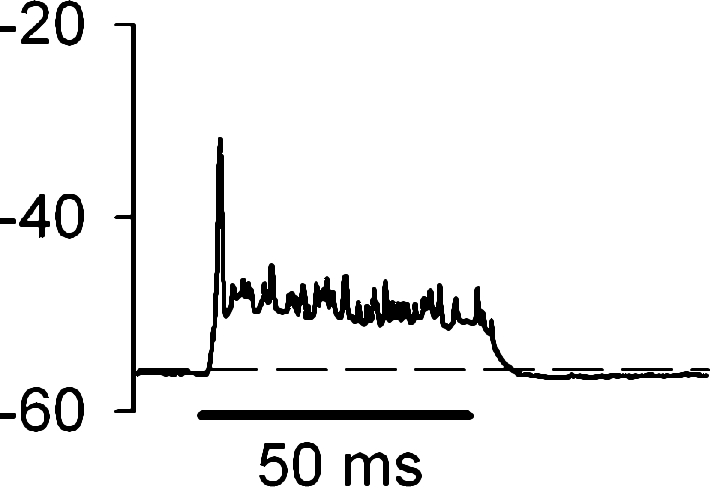
\includegraphics[keepaspectratio,width=0.3\textwidth]{TStellate/CT1-01-857-007}}\hfill%\\
\subfloat[Chopper Transient 2]{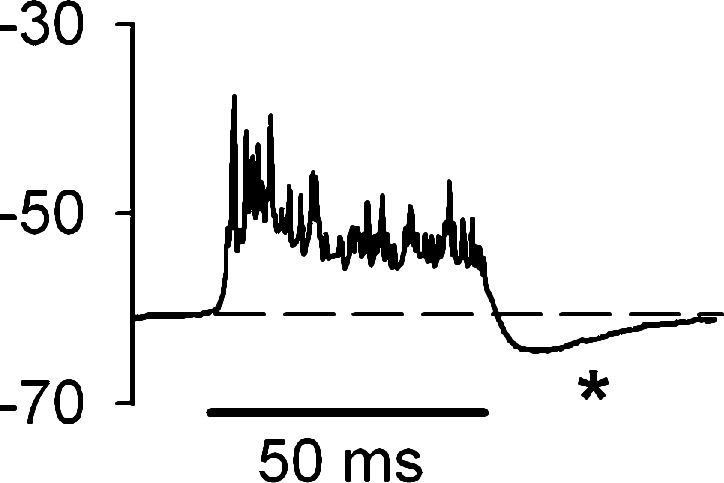
\includegraphics[keepaspectratio,width=0.3\textwidth]{TStellate/CT2-01-305-014}}%\quad%
%\subfloat[Onset Chopper]{\resizebox{0.35\textwidth}{!}{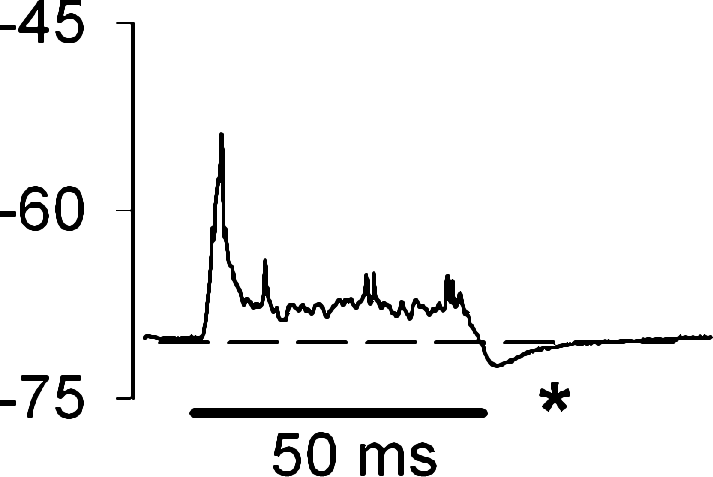
\includegraphics{TStellate/OC-99-812-013}}}
\caption[Average intracellular response data in stellate cells in rats.]{Average intracellular response to CF tone 30dB above depolarisation threshold in stellate  cells~\citep[Reproduced from Fig.~2, ][]{PaoliniClareyEtAl:2005}.
A. Sustained chopper unit 01-864-004, CF 3.8~kHz,
B. Transient chopper type 1 unit 01-857-007, CF 8.9~kHz.
C. Transient chopper type 2 unit 01-305-014 CF 12.3~kHz.
%D. Onset chopper unit  99-812-013.
Hyper polarisation after tone indicated by asterisk.  \label{fig:PaoliniAIV}}
\end{figure}
\yellownote{Permission needed for Paolini plots}

The categorisation via coefficient of variation is shown in Figure~\ref{fig:PaoliniCVdata}.
Sustained choppers maintain a stable CV below 0.2 throughout the entire stimulus. The transient chopper optimisation had two types defined by \citep{PaoliniClareyEtAl:2005}.
The first CT type is categorised with CV starting below 0.2 then rising, hence the name transient, but stays below 0.3.
The second CT type is regular in the first 10 ms period, but rises to 0.3 or above throughout the stimulus.

\begin{figure}[htb]
\centering%
%\resizebox{0.6\textwidth}{!}{
\includegraphics{TStellate/PaoliniCV.eps}
%}
\caption{Regularity in chopper units \citep[Data reproduced from Fig.~2,~][]{PaoliniClareyEtAl:2005}}
\label{fig:PaoliniCVdata}
\end{figure}


\subsection{Implementation}

\yellownote{Para 1: Nordlie table~\ref{tab:TSModelSummary}A. Using R\&M  type I-t, Other previous models}
\yellownote{Synaptic inputs known and unknown, included and not included in model.  Previous work include and excludes}

Figure~\ref{fig:TSinputs} shows the expected response of a T~stellate cell to individual connections from different cells in the CN stellate network.
The membrane parameters for the single compartment T~stellate cell model are default except for sodium conductance set to zero.
In this example, excitation from the afferent \ANF~inputs (\LSR~Figure~\ref{fig:TSinputs}A and \HSR~Figure~\ref{fig:TSinputs}B) show a large depolarisation.
\HSR~inputs show a rapid onset and a slowly adapting sustained depolarisation.


\yellownote{Actual parameters: diameter =19.5$\mu$m, $\gNa=0$, $\gKHT=0.0189416$ S cm$^{-2}$, $\gleak=0.000473539$ S cm$^{-2}$, $\gh=$6.20392e-05 S cm$^{-2}$, $\gKA=0.01539$ S cm$^{-2}$, $\Eleak=-65$ mV, $\ENa=50$ mV, $\EK=-70$ mV.}


\begin{figure}[htb]
\centering%
\includegraphics[keepaspectratio,width=0.9\textwidth]{TStellate/baseline_exc}\\
\includegraphics[keepaspectratio,width=0.9\textwidth]{TStellate/baseline_inh}
\caption[Response of T~stellate cells to isolated synaptic inputs]%
{Intracellular membrane voltage response of a T~stellate cell model to isolated synaptic inputs.
A pure tone stimulus of 8.2~kHz at 85 dB~SPL was presented to the CN network. The CF of the recorded TS unit was 8.267~kHz.
Single stimulus responses are shown as a thin line and average response over 25 repetitions is shown as the dark line.
A. 30 LSR ANF synapses.
B. 20 HSR ANF synapses.
C. 20 D stellate cell glycinergic synapses.
D. 15 Golgi cell \GABAa synapses.
All weights were set to $0.0005\,\mu{\rm S}$ and the sodium conductance (\gNa)set to zero.
The parameters for synapse's were: excitatory (tau = 0.36 ms), glycinergic (tau1=0.4 and tau2=2.5 ms), and GABAergic (tau1=0.26 and tau2=5.43 ms).\label{fig:TSinputs}}
\end{figure}

\begin{figure}[htb]
\centering%
% \resizebox{0.9\textwidth}{!}{\includegraphics{TStellate/baseline_jitter}}
\includegraphics[keepaspectratio=true,width=0.9\textwidth]{TStellate/baseline_jitter}
  % \caption[Response of T~stellate cells to isolated synaptic
  % inputs]{Intracellular membrane voltage response of a T~stellate cell
  %   model to isolated synaptic inputs. A pure tone stimulus of 8.2~kHz at
  %   85 dB~SPL was presented to the CN network. The CF of the recorded
  %   T~stellate cell was 8.267~kHz.  Single stimulus responses are shown as
  %   a thin line and average response over 25 repetitions is shown as the
  %   dark line. A. 30 LSR ANF synapses. B. 20 HSR ANF synapsexs. C. 20 D
  %   stellate cell glycinergic synapses. D. 15 Golgi cell GABA$_{\rm A}$
  %   synapses. All weights were set to $0.0005\,\mu{\rm S}$ and the sodium
  %   conductance set to zero.  The parameters for synapases were: excitatory
  %   (tau = 0.36 ms), glycinergic (tau1=0.4 and tau2=2.5 ms), and
  %   GABAergic (tau1=0.26 and tau2=5.43 ms).\label{fig:TSExcinputs}}
\caption[]{Jitter of AN input T~stellate Optimisation results}\label{fig:CSjitter}
\end{figure}



\clearpage
\subsection{Optimisation Results}

\yellownote{Choosing optimisation data - average population data or individual exemplar based on Paolini rat data.}


What is not shown in Figure~\ref{fig:TSinputs} is firstly the non-linear dynamics of the action potential in the neural model; and secondly the hyperpolarisation activation of I$_{\rm h}$ and I$_{\rm KA}$ currents due to inhibitory input.
The second factor is important in enhancing the first spike response across the T~stellate cells \citep{PaoliniClareyEtAl:2004} to an oncoming stimulus, since the \OnC~units will respond earlier and provide fast inhibition.

%       \begin{figure}[htb]
%         \centering\resizebox{0.95\textwidth}{!}{%
%           \includegraphics{RateLevel/psthsingle90.0.eps}%
% %          \includegraphics{RateLevel/TS_ratelevel.eps}}
%       \end{figure}

The final error for the optimisation routine was calculated as the square root of the mean squared error between the first 4 CV periods and the three voltage measures.
The measures of membrane voltage were independent of \RMP included a) the onset ratio ($v_{\rm 5-10}/v_{\rm 20-30}$), b) adaptation of sustained depolarisation ($v_{\rm 20-21} - v_{\rm 50-51}$), and c) post-tone hyperpolarisation ($v_{\rm RMP} - v_{\rm 60-61}$).


\subsubsection{Sustained Chopper}

Figure~\ref{fig:CSresults} shows the optimisation results for the sustained chopper (CS) unit 01-864-004 from \citep{PaoliniClareyEtAl:2005}, with CF 3.9~kHz.
This unit had a depolarisation threshold at 10 dB and a firing rate saturation at 75 dB SPL.
The stimulus for the optimisation routine was a pure tone 30~dB above depolarisation threshold at CF (3.9~kHz 40~dB SPL), 5 ms on/off cosine squared ramp.
A 20 ms delay was included to allow the model to reach a sustained \RMP. The CS model unit had CF of 3.872~kHz due to the separation of frequency channels in the model.
The best parameters found by the optimisation and shown in Figure~\ref{fig:CSresults}, were very high excitatory input (\wLSRTS 0.00286796, \wHSRTS 0.00201089) and moderate to high inhibition (\wDSTS 0.000291181, \wTVTS 0.000884174, \wGLGTS 0.000749812).
A low input stimulus level means that the majority of synaptic input came from \HSR fibres.
There was a slight increase in the leak conductance (\gleak=6.57345e-4 Scm$^-2$ ) from the initial value (4.907e-4), causing a decrease in the input resistance to 120~M$\Omega$ from 163~M$\Omega$.
The final error, calculated with more weight on the CV variables, was 0.839952.
Post-tone hyperpolarisation (reference 1.30035, best CS model -0.029843) and the first CV value (ref 0.1543, best CS model 0.49706) had the greatest difference.
The poor initial CV response is due to the irregular first spike.
The large excitatory \HSR input causes spikes occurring after tone onset, just before the stimulus invoked spike arrival at the TS cell 3 ms later, but still included in the CV calculation.


\yellownote{Note the CS optimisation had added weight to the CV values in the error calculation.  The PSTH and IV trace do not even show a decent chopping behaviour.}
\yellownote{The peaks for the IV are 3.66, 6.77, and 10.99
  ms. The AN model input is affected by the rat audiogram, the low CF and low level.  This shifts the arrival time of spikes to the TS model, and a raw IV comparison would need to be shifted by approx 2 ms.  The onset ratio and the first CV value are effected by this.}
\yellownote{Synaptic weight in the model above 0.002 will initiate a spike at each input spike, similar to the calyx synapse on bushy cells. This means that the TS cell will respond with a primary-like or primary with notch   PSTH. Dendritic filtering could improve this but the high synaptic weights do   not seem like a realistic physiological option for small bouton endings in the CN.}

\begin{figure}[htb]
\centering%
%\resizebox{0.95\textwidth}{!}{}
\includegraphics{/media/data/Work/cnstellate/TStellate_CS/multiplotIVCV.eps}
\caption[CS T~stellate Optimisation results]{Optimisation results for the CS type T~stellate cell.
The reference data for CS unit 01-864-004 from  \citep{PaoliniClareyEtAl:2005}, with CF=3.9~kHz, is shown in blue and the     optimised model is shown in black (CF=3.872 kHz).
The stimulus (pure tone  3.9~kHz stimulus, 40dB SPL)  was repeated 50 times for this figure but during the optimisation routine the  repetition was 25.
A. PSTH B. Coefficient of variation averaged over 10 ms periods.
C. Average membrane voltage (note shaded areas indicate areas used in the measures in D.
D. Measures of membrane voltage including a) onset ratio ($v_{\rm 5-10}/v_{\rm 20-30}$), b) adaptation of sustained depolarisation ($v_{\rm 20-21} - v_{\rm 50-51}$ mV), and c) post-tone hyperpolarisation ($v_{\rm RMP} - v_{\rm 60-61}$ mV).
The final error for the CS unit model was 0.839952, with double weighting for CV values.
The RMP, calculated from -10 to 0 ms, for the reference unit and best parameter model was -45.1 and -64.22, respectively.}
\label{fig:CSresults}
\end{figure}

\yellownote{The RMP of the experimental data was relatively high, and if this was produced in a model the spontaneous rate would be close to 100 spikes per seconds.  The  IV measures allow for comparison of the experimental and model data that is   independent of the RMP.}

\yellownote{Hand tuning creates many types of CS models, but the best effects are when you smooth out the input with dendritic filtering.  This can be used in a   single compartment using a higher time constant on the synapse or better, using a double-exponential synapse with longer onset and decay time   constants. Very high excitatory inputs saturates the cell and it will spike   repeatedly in a regular fashion but the onset is too precise. See CT2 IV trace   for an example of precise onset. I was able to generated a good IV trace when   the full trace was the error function at higher SPL and higher CF, but this   was unable to generate the same trace for 3.9 KHz at 40 dB or a sustained CV. }

\clearpage
\subsubsection{Transient Chopper 1}

The CT1 unit chosen for the optimisation was unit 01-857-007 \citep{PaoliniClareyEtAl:2005} (CF=8.2~kHz).
The depolarisation threshold for this unit was 55~dB, close to the average 47.2~dB for CT1 units.
The stimulus for the optimisation routine was an 85~dB 8.2 kHz pure tone and the exemplar TS cell model had CF 8.27~kHz.

The optimisation results of CT1 ares shown in Figure~\ref{fig:CT1results} with a final error of 0.839141 without weighting.
Moderate excitatory synaptic weights (\wLSRTS 0.000822193, \wHSRTS 0.000620294) is balanced with moderate to low glycinergic synaptic input (\wDSTS 0.000148518, \wTVTS 0.000195416).
The GABAergic input weight was very low (\wGLGTS 1.70742e-05), but the loud input stimulus (85 dB) would cause reasonable inhibition to the TS cell throughout the stimulus.
The leak conductance had a slight decrease (\gleak 0.000409819).


\begin{figure}[htb]
  \centering
%  \resizebox{0.95\textwidth}{!}{\includegraphics{TStellate_CT1/optplot.eps}}
%\resizebox{0.95\textwidth}{!}{\includegraphics{TStellate/TStellate_CT1/multiplotIVCV}}\\
%  \resizebox{0.95\textwidth}{!}{\includegraphics{TStellate_CT1/multiplotIVCV}}
% \resizebox{0.95\textwidth}{!}{
\includegraphics{TStellate_CT1/multiplotIVCV3}
  \caption[CT1 T~stellate Optimisation results]{CT1 T~stellate cell mod optimisation results.
The RMP for the reference unit and best parameter     model was -55.98 and -64.97 mV, respectively.
The final error was 0.839141,     without weighting.
See Figure~\ref{fig:CSresults} for figure configuration.
A. PSTH, B. CV, C. Average membrane voltage, and D. Voltage measures.}
  \label{fig:CT1results}
\end{figure}

\clearpage
\subsubsection{Transient Chopper 2}

The second transiently adapting chopper unit's difference to CT1 is reflected in its average membrane potential and CV.
CT2 has a higher reduction in onset depolarization (90.2\%) compared to CT1, and post-tone inhibition is greater (8.82 mV).
The exemplar CT2 unit (01-305-014, CF 12.4~kHz \citep*{PaoliniClareyEtAl:2005}), has a low depolarising threshold (5 dB) so the stimulus is set to 35 dB SPL. The model TS unit  had a CF of 12.427 kHz.

%    chopper transient type 2
%    // unit 01-305-014 \citep{PaoliniClareyEtAl:2005}
%    //CV (10ms segs) first 10m below 0.2, then rises above 0.3
%    // rate saturation at 5 dB
%    spl      = 35   //30 dB above depolarisation threshold
%    tonefreq = 12400 //Hz

% #RMP	-60.6332	-64.957
% #IVOnset	0.902367	0.962511
% #IVAdaptation	8.82784	7.8878
% #IVOffset	3.24212	2.18856

Fitting data was compared against experimental data of a chopper units in the rat cochlear nucleus \citep{PaoliniClareyEtAl:2005}.
Figure~\ref{fig:CT2results} shows the results of the CT2 optimisation.
The resting membrane potential for the exemplar and model CT2 unit was -60.63 and -64.96 mV for the optimised model and exemplar unit, respectively.


\begin{figure}[htb]
 \centering
%\resizebox{0.95\textwidth}{!}{}
\includegraphics{/media/data/Work/cnstellate/TStellate_CT2/multiplotIVCV}
% \resizebox{0.95\textwidth}{!}{\includegraphics{TStellate_CT2/multiplotIVCV3}}
  \caption[CT2 T~stellate Optimisation results]{CT2 T~stellate Optimisation results.
The RMP for the reference unit and best CT1 model was -60.63 and -64.95 mV, respectively.
See Figure~\ref{fig:CSresults} for figure configuration.
A. PSTH, B. CV, C. Average membrane voltage, and D. Voltage measures.}
  \label{fig:CT2results}
\end{figure}



{\small% % D~----------------------------- -----
\noindent
\begin{tabularx}{\linewidth}{|X|c|c|c|c|c|}
\hdr{6}{F}{Optimisation} \\ \hline
          \textbf{Parameters}           & \textbf{Label} & \textbf{Range} & \multicolumn{3}{|c|}{\textbf{Best Values}}\\
                                        &                &                &      CS     &     CT1     & CT2 \\\hline
   Weight of HSR syn on TS  ($\mu$S)    &    \wHSRTS     &  [1e-5,0.03]   & 0.00201089  & 0.000817015 & 0.00248999 \\
   Weight of LSR syn on TS  ($\mu$S)    &    \wLSRTS     &  [1e-5,0.03]   & 0.00286796  & 0.000774459 & 0.00203762\\ 
   %  Number of synapses, LSR to TS     &    \nLSRTV     &     [0,64]     &             &             & \\                       
   %  Number of synapses, HSR to TS     &    \nHSRTV     &     [0,64]     &             &             & \\
   Weight of DS syn on TS  ($\mu$S)     &     \wDSTS     &  [1e-5,0.03]   & 0.000291181 & 6.38011e-05 & 0.00113529\\
   %Number of DS syn on TS  ($\mu$S)    &     \nDSTS     &     [0,64]     &             &             & \\
   Weight of TV syn on TS  ($\mu$S)     &     \wTVTS     &  [1e-5,0.03]   & 0.000884174 & 6.46063e-05 & 0.000866815\\
   %Number of TV syn on TS  ($\mu$S)    &     \nTVTS     &     [0,64]     &             &             & \\
   Weight of GLG syn on TS  ($\mu$S)    &    \wGLGTS     &  [1e-5,0.03]   & 0.000749812 & 9.3936e-05  & 5e-05\\
  %Number of GLG syn on TS  ($\mu$S)    &    \nGLGTS     &     [0,64]     &             &             & \\ \hline
TS max.\ leak conductance (mS cm$^{-2}$) &     \gleak     &    [1e-3,3]    &  0.657345   &  0.494097   & 0.72474\\
 TS max. KHT conductance (S cm$^{-2}$)  &     \gKHT      &  [1e-6,0.003]	 &  0.0189416  &  0.018941   & 0.022858\\
   %      TS reversal potential (mV)    &     \Eleak     &   [$-45$,$-70$]    &             &   -54.26    & -63.502\\ \hline
                       \multicolumn{3}{|l|}{Error}                        &    6.496    &    5.928    & 5.569\\ \hline
\end{tabularx}
}%\yellownote{Grab most recent data for the table}

\subsection{Verification}

\yellownote{Explain the figure~\ref{fig:TS_verification}}

\begin{figure}[htb]
\centering
\hspace{0.5cm}\figfont{A}\hspace{0.5\textwidth}\figfont{B}\hfill\\
\includegraphics[keepaspectratio=true,width=0.48\textwidth]{ResponsesNoComp/TS_ratelevel_combined.eps}\hfill%
\includegraphics[keepaspectratio=true,width=0.48\textwidth]{ResponsesNoComp/RateLevel/psthsingle90.0.eps}\\
\hspace{0.5cm}\figfont{C}\hspace{0.5\textwidth}\figfont{D}\hfill\\
\includegraphics[keepaspectratio=true,width=0.48\textwidth]{ResponsesNoComp/RateLevel/response_area.0.eps}\hfill%
\includegraphics[keepaspectratio=true,width=0.48\textwidth]{ResponsesNoComp/MaskedResponseCurve3/15/TS_masked.eps}\\
%\resizebox{0.45\textwidth}{!}{\includegraphics{ResponsesNoComp/RateLevel/psthsingle90.3.eps}}\\
%\resizebox{0.45\textwidth}{!}{\includegraphics{ResponsesNoComp/RateLevel/psthsingle50.3.eps}}\\
\caption[Optimised TS cell model responses]{Response of optimised TS cell model at the centre of the network (CF=5.8~kHz). A. Rate level responses to tone, noise and tone plus noise. 
B. PSTH at 90 dB~SPL.  
C. Response area equivalent using all TS units in the network. 
D. Masked response across the CF of the central unit (15 dB masking noise).} \label{fig:TS_verification}
\end{figure}


% \subsubsection{Effect of DS: time frequency enhancement}

% Go on Paolini's proposal

% \subsubsection{Effect of TV: comb filter and echo suppression}


%       \subsection{Tone Response}

%       \begin{figure}[htb]
%         \centering\resizebox{0.95\textwidth}{!}{%
%           \includegraphics{RateLevel/psthsingle90.0.eps}%
% %          \includegraphics{RateLevel/TS_ratelevel.eps}}
%       \end{figure}
%       \begin{figure}[htb]
%         \centering\resizebox{0.95\textwidth}{!}{%
%  %         \includegraphics{RateLevel/response_area.0.eps}%
%   %        \includegraphics{RateLevel/response_area_log2.0.eps}}
%       \end{figure}
%       \begin{figure}[htb]
%         \centering\resizebox{0.95\textwidth}{!}{%
%           % \includegraphics{RateLevel/response_area.0.eps}
%           \includegraphics{RateLevel/psthall90.0.eps}%
%           \includegraphics{RateLevel/psthVlevel.0.eps}}
%       \end{figure}


%       \clearpage
%       \subsection{Noise Response}
%       \begin{figure}[htb]
%         \centering\resizebox{0.95\textwidth}{!}{%
%           \includegraphics{NoiseRateLevel/psthsingle120.0.eps}%
%           \includegraphics{NoiseRateLevel/TS_ratelevel.eps}}
%       \end{figure}
%       \begin{figure}[htb]
%         \centering\resizebox{0.95\textwidth}{!}{%
%           \includegraphics{NoiseRateLevel/response_area.0.eps}%
%           \includegraphics{NoiseRateLevel/response_area_log2.0.eps}}
%       \end{figure}
%       \begin{figure}[htb]
%         \centering\resizebox{0.95\textwidth}{!}{%
%           % \includegraphics{RateLevel/response_area.0.eps}
%           \includegraphics{NoiseRateLevel/psthall90.0.eps}%
%           \includegraphics{NoiseRateLevel/psthVlevel.0.eps}}
%       \end{figure}


%       \clearpage
%       \subsection{Masked Noise and Tone}
%       \begin{figure}[h!]
% \centering\resizebox{0.95\textwidth}{!}{\includegraphics{MaskedRateLevel/psthsingle90.0.eps}\includegraphics{MaskedRateLevel/TS_ratelevel.eps}}
%       \end{figure}
%       \begin{figure}[h!]
%         \centering\resizebox{0.95\textwidth}{!}{%
%           \includegraphics{MaskedRateLevel/response_area.0.eps}%
%           \includegraphics{MaskedRateLevel/response_area_log2.0.eps}}
%       \end{figure}

%       \begin{figure}[h!]
%         \centering\resizebox{0.95\textwidth}{!}{%
%           % \includegraphics{RateLevel/response_area.0.eps}
%           \includegraphics{MaskedRateLevel/psthall90.0.eps}%
%           \includegraphics{MaskedRateLevel/psthVlevel.0.eps}}
%       \end{figure}
%       \clearpage
%       \subsection{Masked Response Area}
%       \begin{figure}[h!]
%         \centering\resizebox{0.95\textwidth}{!}{%
%           \includegraphics{MaskedResponseCurve/psthsingle5810.0.eps}%
%           \includegraphics{MaskedResponseCurve/TS_masked.eps}}
%       \end{figure}
%       \begin{figure}[h!]
%         \centering\resizebox{0.95\textwidth}{!}{%
%           \includegraphics{MaskedResponseCurve/response_area.0.eps}%
%           \includegraphics{MaskedResponseCurve/response_area_log2log2.0.eps}}
%       \end{figure}

%       \begin{figure}[h!]
%         \centering\resizebox{0.95\textwidth}{!}{%
%           % \includegraphics{RateLevel/response_area.0.eps}
%           \includegraphics{MaskedResponseCurve/psthall5810.0.eps}%
%           \includegraphics{MaskedResponseCurve/psthVmod.0.eps}}
%       \end{figure}
%       \clearpage



%%% Local Variables:
%%% mode: latex
%%% mode: tex-fold
%%% mode: visual-line
%%% TeX-master: "SimpleResponses"
%%% TeX-PDF-mode: nil
%%% End:
